% !TEX root =  master.tex
\cleardoublepage
\chapter{Grundlagen des PCR-Poolings}
In diesem Kapitel sollten die Grundlagen und Parameter für das PCR-Pooling beschrieben werden.


\section{Mögliche Poolgrößen und Erkennungsrate}%\newline
Das PCR-Verfahren erlaubt grundsätzlich ein Pooling von mehreren Testpersonen.
Die Proben der Patienten werden hierfür zu einem Pool zusammengefasst und gemeinsam getestet.
Das PCR-Verfahren ist darauf ausgelegt, geringe DNA-Mengen zu einer nachweisbaren Menge zu vermehren.
Die Verwässerung der Probe ist bis zu einem gewissen Punkt deshalb unproblematisch für den Nachweis.
Auch eine (zu) hohe Verdünnung ist zulasten der Erkennungsrate problemlos möglich.
Abgewogen werden muss hierbei die Priorisierung zwischen Präzision und Kostenersparnis.
Eine Poolgröße von bis zu 20 Personen liegt laut Viehweger "comfortable above the detection rate"\footnote{Vieweger v1}
Andere Gruppe halten Poolgrößen von bis zu 90 Personen für akzeptabel.\footnote{Quelle 2 Pooling Verwässerung}

Es ist zu beachten, dass bei größeren Pools mehr Verdopplungsschritte notwendig sind, um dieselbe Virenmenge in der Probe zu erhalten.
Beim Pooling von 16 Personen liegt beispielsweise eine um $2^{4}$ niedrigere Virenlast vor.
Deshalb müssen 4 weitere Zyklen eingeplant werden.
\footnote{Vieweger v1}


\begin{wrapfigure}{r}{0.5\textwidth}
	%\centering
	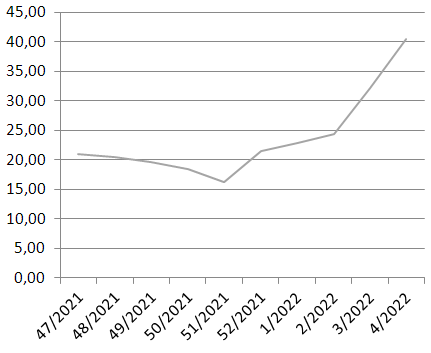
\includegraphics[width=.5\textwidth]{img/RKI_PCR_Positivrate}
	\caption{Positivrate PCR-Tests\footnotemark}
\end{wrapfigure}

\section{Prävalenz}%\newline
Die Prävalenz ist die Quote, mit welcher eine Krankheit in einer Stichprobe vorkommt.\footnote{Leon Gordis S37}
Sie ist ähnlich der derzeit allgemein bekannteren Inzidenz, welche sich auf die Gesamtbevölkerung bezieht.
Bei einer anlasslosen, repräsentativen Testung der Bevölkerung kann die Prävalenz eines Tests gleich der Inzidenz sein.
Bei einer anlassbezogenen Testung werden allerdings meist deutlich höhere Prävalenzen beobachtet.
Gemäß aktuellem RKI-Wochenbereicht sind zwischenzeitlich über 40 Prozent der PCR-Tests positiv.
\footnote{RKI Wochenbericht}

\section{Ergebnisinterpretation und Effizienz}
\begin{itemize}
	\item \textbf{Negatives Poolergebnis:}\newline
	Ein negatives Gesamtergebnis bedeutet, dass \textbf{jede Einzelprobe negativ} war.
	
	Es wurde somit durch einen Test festgestellt, dass alle Personen im Pool negativ sind.
	
	Die Effizienz lässt sich somit beschreiben als $\frac{Anzahl Testpersonen (N)}{Anzahl Tests (1)} $.
	
	\item \textbf{Positives Poolergebnis:}\newline
	Ein positives Gesamtergebnis bedeutet, dass \textbf{mindestens eine Einzelprobe positiv} war.
	
	In diesem Fall müssen weitere Tests durchgeführt werden, um die positiven Einzelpersonen zu ermitteln.
	Die Tests erfolgen hierbei nacheinander und sind statistisch unabhängig voneinander.
	
	Die Nachtestung kann durch mehrstufiges Pooling optimiert werden.
	Für das einfachste Basisverfahren wird allerdings angenommen, dass nach einem Positivergebnis das Pooling beendet wird.
	Die Personen innerhalb des positiven Pools werden einzeln nachgetestet.\footnote{Viehweger Zeile 11}
	
	Im Falle einer Nachtestung wird somit ein initialer Test für den Pool benötigt, welcher positiv ausfällt.
	Danach werden nochmal Tests für jede Einzelperson benötigt.
	Die Effizienz lässt sich somit beschreiben als $\frac{Anzahl Testpersonen (N)}{1 Pooltest + N Einzeltests} $.
	Die Testung erfolgt zweistufig.
	
\end{itemize}

\section{Unklare Ergebnisse und Nachtestung}%\newline
Durch Pooling besteht das Risiko, dass die Ergebnisse nicht für alle Testpersonen eindeutig interpretiert werden können.
Hierdurch kann eine Nachtestung erforderlich werden.
Wie häufig dies der Fall ist und welcher Anteil der Testgruppe nachuntersucht werden muss, ist abhängig vom gewählten Verfahren.
Die Proben müssen ausreichend umfangreich sein, um genug Substanz für mehrere Testungen zu enthalten.

Durch die erneute Testung verlängert sich der Zeitraum, bevor für alle Testpersonen das Ergebnis fest steht.
Dies kann abhängig von der Situation in welcher der Test benötigt wird nicht akzeptabel sein.
Manche Verfahren erfordern sogar mehrere sequenzielle Nachtestungen.

\section{Verhinderung von Kontamination}%\newline
Beim Pooling des ersten Durchlaufs muss darauf geachtet werden, die Proben untereinander nicht zu kontaminieren.
Eine verunreinigung der Originalproben würde eine spätere Nachtestung unmöglich machen.

Um eine Kontamination durch das Pooling zu verhindern, sollte die komplette Matrix vor dem Pooling einmal dupliziert werden. 
Die für den aktuellen Test notwendigen Proben werden hierbei entnommen und im Duplikat gepoolt.
Für diesen Duplikationsschritt gibt es spezialisierte Laborgeräte, sodass dies in einem Arbeitsschritt für alle Proben durchgeführt werden kann.\footnote{https://www.genengnews.com/wp-content/uploads/2019/07/Eppendorf.jpg}

\begin{figure}[h]
	\centering
	
\includegraphics[width=.45\textwidth]{img/Pipettenmatrix}
	\caption{Pipettenautomat\footnotemark}
\end{figure}


\section{Sicherheitsniveaus}

An dieser Stelle ist zu bemerken, dass es innerhalb der Testgruppe drei Kategorien von Testergebnis gibt.
\begin{itemize}
	\item \textbf{2x Positiv} Bei Probe 3-2 (rot) sind als einziges beide Pooltests A2 und B3 positiv ausgefallen. Diese Person ist höchstwahrscheinlich positiv und wird einzeln nachgetestet.
	\item \textbf{1x Positiv} 6 Proben (hellrot) weisen ein positives und ein negatives Ergebnis auf.
	\item \textbf{beide negativ} Bei den verbleibenden Personen (grün) sind zwei unabhängige Pooltests negativ. Sie sind höchstwahrscheinlich nicht infiziert.
\end{itemize}
Hieraus ergibt sich nun die Frage, welcher Sicherheitsanspruch gegenüber dem Test erhoben wird.
Eine Person mit zwei positiven Testergebnissen ist höchstwahrscheinlich infiziert und wird in jedem Fall einzeln nachgetestet.
Eine Person mit zwei negativen Testergebnisen ist höchstwahrscheinlich nicht infiziert und bekommt ein negatives Testzertifikat.
Wie sollte man nun mit den Personen verfahren, die Teil eines positiven Pools waren?

\begin{itemize}
	\item \textbf{Hohes Sicherheitsniveau} Alle zweifelhaften Personen werden einzeln nachgetestet.
	\item \textbf{Mittleres Sicherheitsniveau} Alle zweifelhaften Personen werden in einen eindimensionalen Pool kombiniert und gemeinsam getestet. Hierdurch kann ermittelt werden, ob beim ersten Durchlauf Fehler passiert sind und Personen übersehen wurden. Im Falle eines Positiven Poolergebnisses müssen alle einzeln nachgetestet werden. Hierduch werden drei sequenzielle Durchläufe notwendig, was die Übermittlung des Testergebnisses inakzeptabel lang verzögern kann.
	\item \textbf{Geringes Sicherheitsniveau} Die Personen für welche es keine Überschneidung gibt, werden als negativ gewertet. In einer perfekten Modellwelt mit 100 Prozent genauen Tests und keinen Anwendungsfehlern wäre auch dies unproblematisch. In der Realität können hierdurch aber falsch-negative Ergebnisse übermittelt werden.
\end{itemize}

\section{Mehrere Positivfälle}

Schwieriger wird es zudem, wenn mehrere Personen innerhalb des Pools positiv sind.
Die Positiven Tests lassen sich dann nicht mehr exakt einer Person zuordnen.
Die beiden positiven Personen (1-4 und 3-2) in Abb 3.3 lösen die Tests A2, A4, B1 und B3 aus.
Neben den positiven Personen zeigen diese Tests auch auf die eigentlich negativen Proben 1-2 und 3-4.
Aus diesem Grund müssen hier für zwei positive Personen vier Proben nachgetestet werden.

\begin{figure}[h]
	\centering
	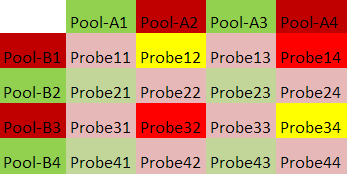
\includegraphics[height=.25\textwidth]{img/2d_Pool_2Positiv}
	\caption{Zweidimensionaler Pool mit zwei positiven Personen (rot). Es treten zwei False-Positives auf (gelb).\footnotemark}
\end{figure}

Grundsätzlich verhält sich der Bedarf an Nachtestungen quadratisch zur Anzahl der Positiven Personen.
Es ist allerdings möglich, dass mehrere positive Personen in einem Test sind.
Durch diese Überschneidung verringert sich der Bedarf für Nachtestungen, weswegen eine Clusterung positiver Tests vorteilhaft sein kann.


\cleardoublepage
